%%%%%%%%%%%%%%%%%%%%%%%%%%%%%%%%%%%%%%%%%%%%%%%%%%%%%%%%%%%%%%%%%%%%%%%%%%%%%%%%%%%%%%%%% 
%%%%%%%%%%%%%%%%%%%%%%%%%%%%%%%%%%%%%% Preambule %%%%%%%%%%%%%%%%%%%%%%%%%%%%%%%%%%%%%%%%%
%%%%%%%%%%%%%%%%%%%%%%%%%%%%%%%%%%%%%%%%%%%%%%%%%%%%%%%%%%%%%%%%%%%%%%%%%%%%%%%%%%%%%%%%%%

\documentclass[a4paper, 12pt, leqno]{article}\usepackage[]{graphicx}\usepackage[]{color}
%% maxwidth is the original width if it is less than linewidth
%% otherwise use linewidth (to make sure the graphics do not exceed the margin)
\makeatletter
\def\maxwidth{ %
  \ifdim\Gin@nat@width>\linewidth
    \linewidth
  \else
    \Gin@nat@width
  \fi
}
\makeatother

\definecolor{fgcolor}{rgb}{0.345, 0.345, 0.345}
\newcommand{\hlnum}[1]{\textcolor[rgb]{0.686,0.059,0.569}{#1}}%
\newcommand{\hlstr}[1]{\textcolor[rgb]{0.192,0.494,0.8}{#1}}%
\newcommand{\hlcom}[1]{\textcolor[rgb]{0.678,0.584,0.686}{\textit{#1}}}%
\newcommand{\hlopt}[1]{\textcolor[rgb]{0,0,0}{#1}}%
\newcommand{\hlstd}[1]{\textcolor[rgb]{0.345,0.345,0.345}{#1}}%
\newcommand{\hlkwa}[1]{\textcolor[rgb]{0.161,0.373,0.58}{\textbf{#1}}}%
\newcommand{\hlkwb}[1]{\textcolor[rgb]{0.69,0.353,0.396}{#1}}%
\newcommand{\hlkwc}[1]{\textcolor[rgb]{0.333,0.667,0.333}{#1}}%
\newcommand{\hlkwd}[1]{\textcolor[rgb]{0.737,0.353,0.396}{\textbf{#1}}}%

\usepackage{framed}
\makeatletter
\newenvironment{kframe}{%
 \def\at@end@of@kframe{}%
 \ifinner\ifhmode%
  \def\at@end@of@kframe{\end{minipage}}%
  \begin{minipage}{\columnwidth}%
 \fi\fi%
 \def\FrameCommand##1{\hskip\@totalleftmargin \hskip-\fboxsep
 \colorbox{shadecolor}{##1}\hskip-\fboxsep
     % There is no \\@totalrightmargin, so:
     \hskip-\linewidth \hskip-\@totalleftmargin \hskip\columnwidth}%
 \MakeFramed {\advance\hsize-\width
   \@totalleftmargin\z@ \linewidth\hsize
   \@setminipage}}%
 {\par\unskip\endMakeFramed%
 \at@end@of@kframe}
\makeatother

\definecolor{shadecolor}{rgb}{.97, .97, .97}
\definecolor{messagecolor}{rgb}{0, 0, 0}
\definecolor{warningcolor}{rgb}{1, 0, 1}
\definecolor{errorcolor}{rgb}{1, 0, 0}
\newenvironment{knitrout}{}{} % an empty environment to be redefined in TeX

\usepackage{alltt} %leqno: numéro d'équation à gauche
\pagenumbering{arabic} % choose how to number the pages
\usepackage{a4wide}
%\usepackage[utf8]{inputenc} % accents interprétés
\usepackage{graphicx}
%\usepackage{subfig}
%\usepackage[hmargin=2cm, vmargin = 2cm, noheadfoot]{geometry} %% Pour gérer le format des pages
%\usepackage{layout} %% Pour avoir la longueur des marges
\usepackage[round,sort]{natbib} %% Natbib is a popular style for formatting references.
%\usepackage{multibib}
%\newcites{secnm}{Bibliographie} 
\usepackage{verbatim} % for multiline comments
\usepackage{amssymb} %symbole de maths
\usepackage{amsmath} %idem
%\usepackage{stmaryrd} %% Symbole flèche à l'envers
\usepackage{amsfonts}
\usepackage[francais,english]{babel} %% Les titres en anglais
\usepackage[utf8]{inputenc} % accents interprétés
\usepackage{array} %% Pour centrer verticalement le contenu d'un tableau, entre autres...
\setcounter{secnumdepth}{4} %% Profondeur des sections, subsections
\usepackage{setspace} %% Gère l'interligne: singlespacing, doublespacing
\singlespacing
\usepackage[colorlinks=true,citecolor=blue]{hyperref} %% Gère les hyperliens
%\usepackage{textcomp} %% Symbole pourmille
\usepackage{lineno} %% Numérotation des lignes
\usepackage{longtable}
\setlength{\LTleft}{-5cm plus 1 fill}
\setlength{\LTright}{-5cm plus 1 fill}
\usepackage{booktabs}
%\usepackage{colortabs} % can't be found
\usepackage{xcolor}
\usepackage{colortbl} %% color text and table rows
%\usepackage{arydshln} %% dashlines for tabular
%\usepackage{sidecap}
\newcommand{\logit}{\text{logit}}
\newcommand{\bs}[1]{\boldsymbol{#1}}
\newcommand{\p}{\text{p}}
% For changes in tables
\newcommand{\SetRowColor}[1]{\noalign{\gdef\RowColorName{#1}}\rowcolor{\RowColorName}}
\definecolor{gray90}{gray}{0.9}
\newcommand{\mymulticolumn}[3]{\multicolumn{#1}{>{\columncolor{gray90}}#2}{#3}}
\newcommand{\sizeBigTable}{\fontsize{9pt}{9pt}\selectfont}

\newcolumntype{L}[1]{>{\raggedright\let\newline\\\arraybackslash\hspace{0pt}}p{#1}}
\newcolumntype{C}[1]{>{\centering\let\newline\\\arraybackslash\hspace{0pt}}p{#1}}
\newcolumntype{R}[1]{>{\raggedleft\let\newline\\\arraybackslash\hspace{0pt}}p{#1}}

%%%%%%%%%%%%%%%%%%%%%%%%%%%%%%%%%%%%%%%%%%%%%%%%%%%%%%%%%%%%%%%%%%%%%%%%%%%%%%%%%%%%%%%%%%
%%%%%%%%%%%%%%%%%%%%%%%%%%%%%%%%%%%%%% Title %%%%%%%%%%%%%%%%%%%%%%%%%%%%%%%%%%%%%%%%%%%%%
%%%%%%%%%%%%%%%%%%%%%%%%%%%%%%%%%%%%%%%%%%%%%%%%%%%%%%%%%%%%%%%%%%%%%%%%%%%%%%%%%%%%%%%%%%

\title{Hierarchical Bayesian species distribution models with the \textbf{hSDM} R Package}
\date{}
\author{}

%%%%%%%%%%%%%%%%%%%%%%%%%%%%%%%%%%%%%%%%%%%%%%%%%%%%%%%%%%%%%%%%%%%%%%%%%%%%%%%%%%%%%%%%%%
%%%%%%%%%%%%%%%%%%%%%%%%%%%%%%%%%%%%%% Knitr %%%%%%%%%%%%%%%%%%%%%%%%%%%%%%%%%%%%%%%%%%%%%
%%%%%%%%%%%%%%%%%%%%%%%%%%%%%%%%%%%%%%%%%%%%%%%%%%%%%%%%%%%%%%%%%%%%%%%%%%%%%%%%%%%%%%%%%%

%\VignetteEngine{knitr::knitr}
%\VignetteIndexEntry{User manual for hSDM R package}

%%%%%%%%%%%%%%%%%%%%%%%%%%%%%%%%%%%%%%%%%%%%%%%%%%%%%%%%%%%%%%%%%%%%%%%%%%%%%%%%%%%%%%%%%%
%%%%%%%%%%%%%%%%%%%%%%%%%%%%%%%%%%%%%% Document %%%%%%%%%%%%%%%%%%%%%%%%%%%%%%%%%%%%%%%%%%
%%%%%%%%%%%%%%%%%%%%%%%%%%%%%%%%%%%%%%%%%%%%%%%%%%%%%%%%%%%%%%%%%%%%%%%%%%%%%%%%%%%%%%%%%%
\IfFileExists{upquote.sty}{\usepackage{upquote}}{}

\begin{document}
\maketitle
\vspace{-1cm}
\begin{center}
  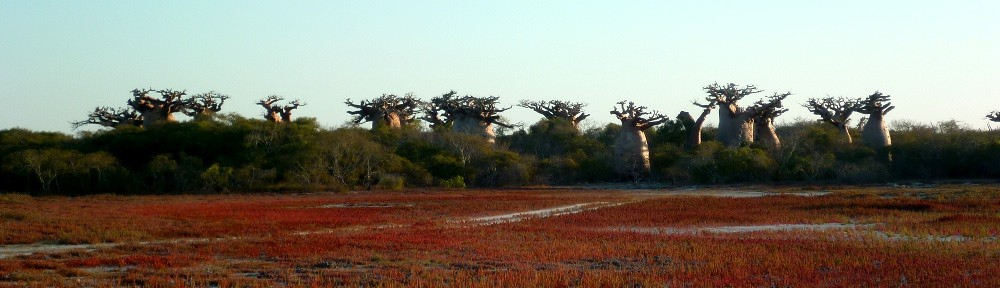
\includegraphics[width=\textwidth]{figures/header.jpg}
\end{center}
\vspace{1cm}
\begin{center}
  \large{Ghislain Vieilledent$^{\star,1}$}
\end{center}

\vspace{0.3cm}

%% {\footnotesize
%% \begin{flushleft}
%%   \textbf{Type of article:} Data paper for \textit{Annals of Forest Science}\\
%%   \textbf{Thematic issue:} GlobAllomeTree web platform\\
%%   \textbf{Running title:} Cirad wood density data base\\
%%   \textbf{Number of words and objects:} whole manuscript (X words) with abstract (X words),
%%   main text (X words), references (X, X words), table and figure legends (X, X words)\\
%% \end{flushleft}}

%\vspace{0.2cm}

{\footnotesize
  \begin{flushleft}
    $[\star]$ \textbf{Corresponding author:}
    \textbackslash{E-mail}:~ghislain.vieilledent@cirad.fr
    \textbackslash{Phone}:~+33.(0)4.67.59.37.51
    \textbackslash{Fax}:~+33.(0)4.67.59.39.09\\
    $[1]$ \textbf{Cirad} -- UPR BSEF, F–34398 Montpellier, France\\
\end{flushleft}}

\newpage
%\doublespacing
%\linenumbers

\renewcommand{\abstractname}{Abstract}
\newcommand{\keywords}[1]{\par\noindent
{\small{\em Keywords\/}: #1}}

\begin{abstract}

  Work in progess...
  
  \vspace{0.5cm}

  \keywords{R}

\end{abstract}

\newpage

%%=============================
%% Change default shunk options



\section{Introduction}

\section{Species distribution models}

\subsection{Binomial model}

\subsubsection{Data generation}

For data generation, we can import virtual altitude data in R. Altitude will be used as an
explicative variable to determine the habitat suitability of a virtual species through a
probability of presence. Altitudinal data are available on the website of the
\textbf{hSDM} R package hosted on Sourceforge
(\url{http://hsdm.sourceforge.net/altitude.csv}).

These data can be transformed into a raster using function \texttt{rasterFromXYZ()} of the
\textbf{raster} package. The raster has 2500 cells (50 columns and 50 rows) and the
altitude is comprised roughly between 100 and 600~m (Fig.~\ref{fig:Altitude}). For
logistic regression, explicative variables are usually centered and scaled to facilitate
the inference of model parameters.

\begin{knitrout}\small
\definecolor{shadecolor}{rgb}{0.969, 0.969, 0.969}\color{fgcolor}\begin{kframe}
\begin{alltt}
\hlcom{# Import altitudinal data}
\hlkwd{library}\hlstd{(raster)}
\hlstd{fname} \hlkwb{<-} \hlstr{"http://hsdm.sourceforge.net/altitude.csv"}
\hlstd{alt.df} \hlkwb{<-} \hlkwd{read.csv}\hlstd{(fname,}\hlkwc{header}\hlstd{=}\hlnum{TRUE}\hlstd{)}
\hlstd{alt.orig} \hlkwb{<-} \hlkwd{rasterFromXYZ}\hlstd{(alt.df)}
\hlkwd{plot}\hlstd{(alt.orig)}
\hlcom{# Center and scale altitudinal data}
\hlstd{alt} \hlkwb{<-} \hlkwd{scale}\hlstd{(alt.orig,}\hlkwc{center}\hlstd{=}\hlnum{TRUE}\hlstd{,}\hlkwc{scale}\hlstd{=}\hlnum{TRUE}\hlstd{)}
\hlkwd{plot}\hlstd{(alt)}
\end{alltt}
\end{kframe}
\end{knitrout}


\begin{figure}[!h] 
  \begin{tabular}{cc}
    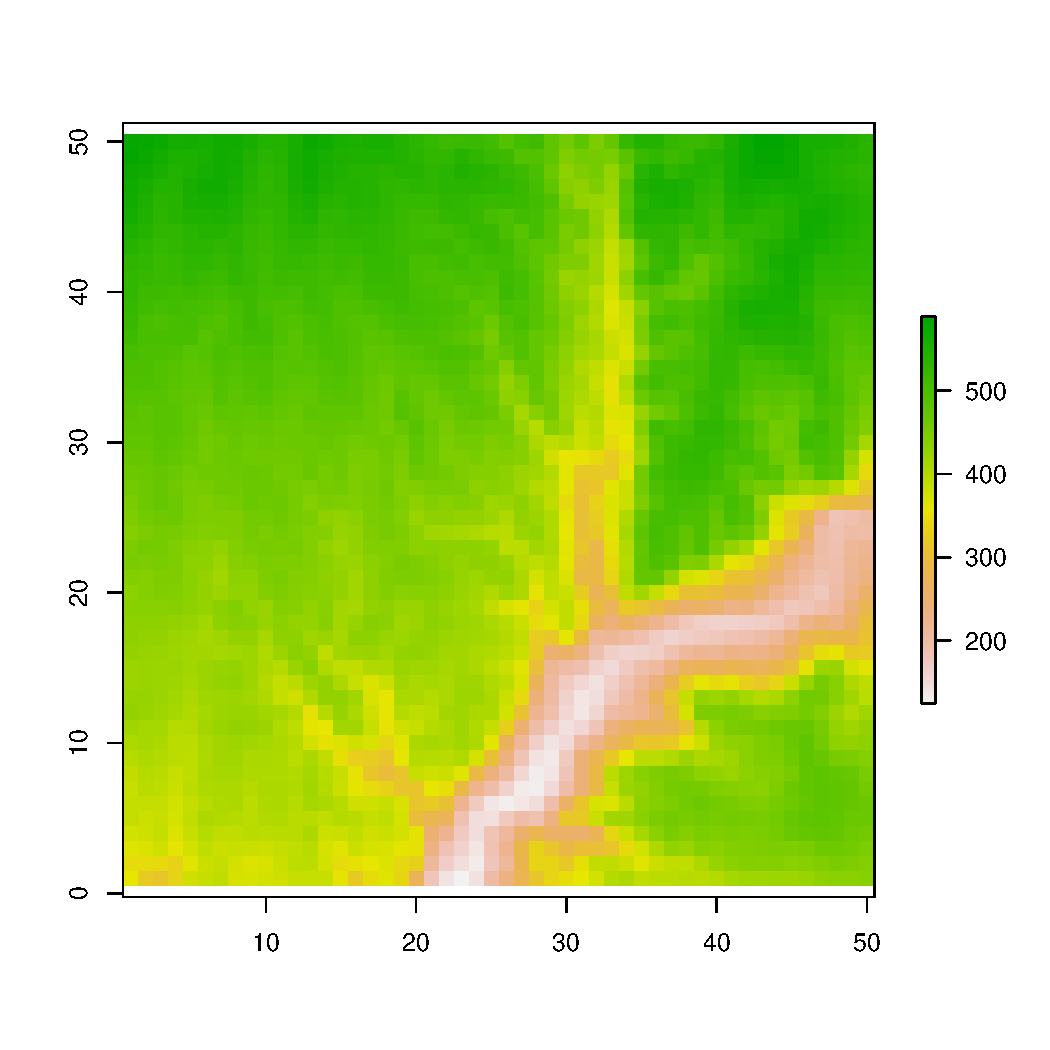
\includegraphics[width=8cm]{figures/Altitude1.pdf} &
    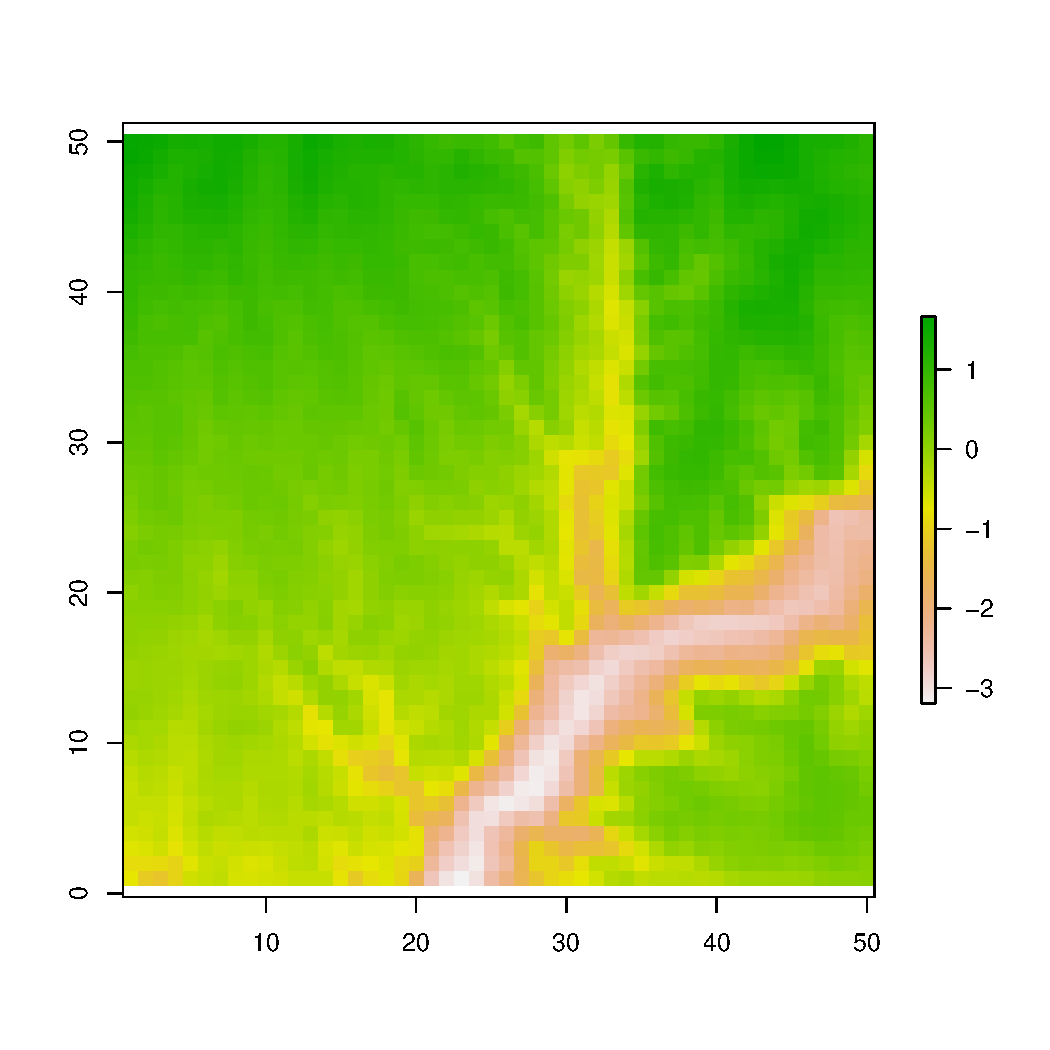
\includegraphics[width=8cm]{figures/Altitude2.pdf} \\
  \end{tabular}
  \caption{\textbf{Altitudinal data}. Original values (in m) on the left. Centered and
    scaled values on the right.}
  \label{fig:Altitude}
\end{figure}

Using the altitude data we can simulate the presence of the virtual species using a
Binomial distribution. We arbitrarily set the trials of the Binomial distribution to
1. Thus, the random variable $y$ representing the presence of the species, follows a
Bernoulli distribution of probability $\theta$. A quadratic effect of the altitude
(variable denoted $x$) is used to compute the probability of presence of the species
using a logit link function (Eq.~\ref{eq:binomial}).

\begin{equation}
  \begin{tabular}{c}
    $y_i \sim \mathcal{B}ernoulli(\theta_i)$ \\
    ~ \\
    $\logit(\theta_i) = \beta_0 + \beta_1 x_i + \beta_2 x_i^2$ \\
  \end{tabular}
  \label{eq:binomial}
\end{equation}

Using matrix notation, the linear model can be written $\logit(\theta_i) = X \beta$. We
fix the parameters to $\beta_0=1$, $\beta_1=2$ and $\beta_2=-4$. The species has a
higher probability of presence at intermediate altitude (Fig.~\ref{fig:theta-binomial}).

\begin{knitrout}\small
\definecolor{shadecolor}{rgb}{0.969, 0.969, 0.969}\color{fgcolor}\begin{kframe}
\begin{alltt}
\hlcom{# Load hSDM library}
\hlkwd{library}\hlstd{(hSDM)}
\hlcom{# Target parameters}
\hlstd{beta.target} \hlkwb{<-} \hlkwd{matrix}\hlstd{(}\hlkwd{c}\hlstd{(}\hlnum{1}\hlstd{,}\hlnum{2}\hlstd{,}\hlopt{-}\hlnum{4}\hlstd{),}\hlkwc{ncol}\hlstd{=}\hlnum{1}\hlstd{)}
\hlcom{# Matrix of covariates (including the intercept)}
\hlstd{X} \hlkwb{<-} \hlkwd{cbind}\hlstd{(}\hlkwd{rep}\hlstd{(}\hlnum{1}\hlstd{,}\hlkwd{ncell}\hlstd{(alt)),}\hlkwd{values}\hlstd{(alt),(}\hlkwd{values}\hlstd{(alt))}\hlopt{^}\hlnum{2}\hlstd{)}
\hlcom{# Probability of presence as a quadratic function of altitude}
\hlstd{logit.theta} \hlkwb{<-} \hlstd{X} \hlopt \hlstd{beta.target}
\hlstd{theta} \hlkwb{<-} \hlkwd{inv.logit}\hlstd{(logit.theta)}
\hlcom{# Transform the probability of presence into a raster}
\hlstd{theta} \hlkwb{<-} \hlkwd{rasterFromXYZ}\hlstd{(}\hlkwd{cbind}\hlstd{(}\hlkwd{coordinates}\hlstd{(alt),theta))}
\hlcom{# Plot the probability of presence}
\hlkwd{plot}\hlstd{(theta,}\hlkwc{col}\hlstd{=}\hlkwd{rev}\hlstd{(}\hlkwd{heat.colors}\hlstd{(}\hlnum{255}\hlstd{)))}
\end{alltt}
\end{kframe}
\end{knitrout}


\begin{figure}[!h] 
  \centering 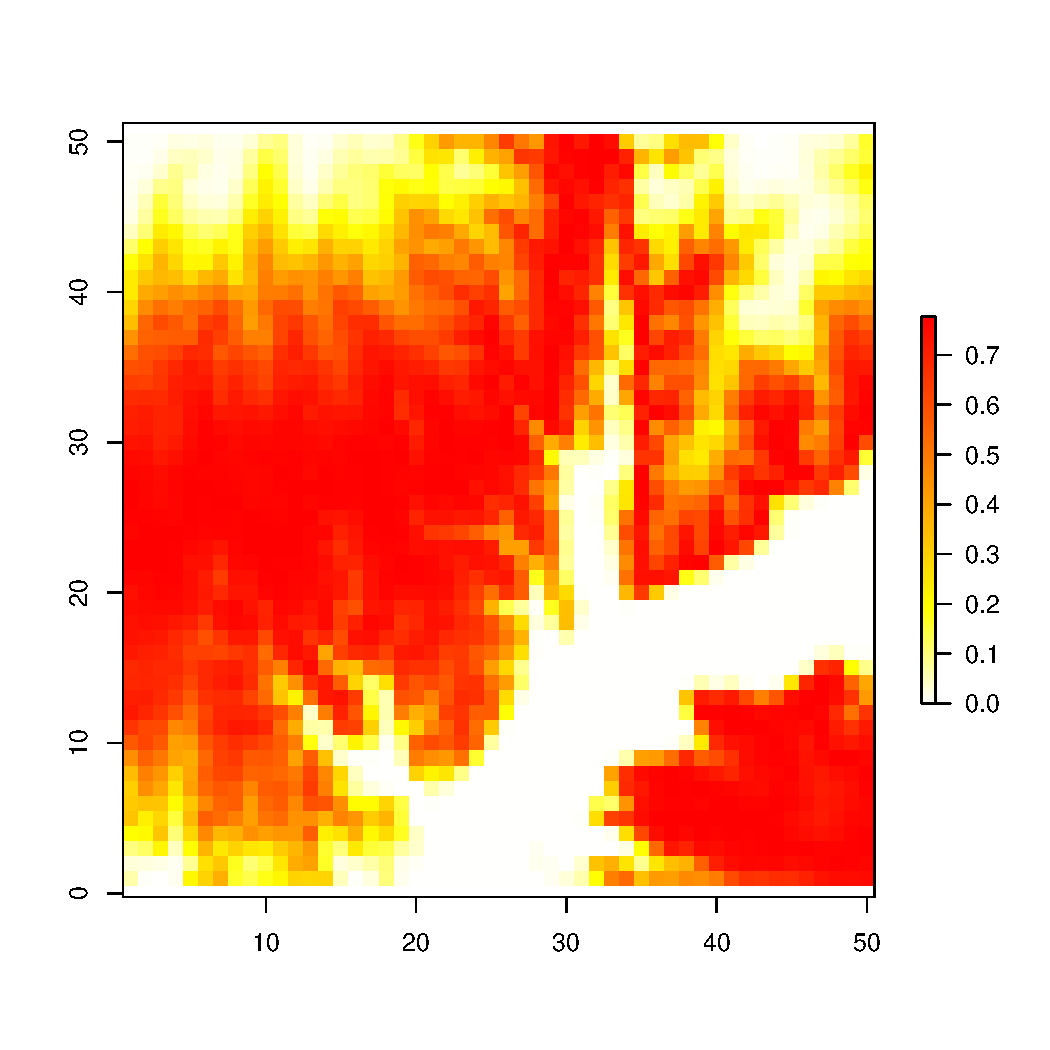
\includegraphics[width=8cm]{figures/theta-binomial.pdf}
  \caption{\textbf{Probability of presence}.}
  \label{fig:theta-binomial}
\end{figure}

We can assume a number $n$ of points in the landscape where we have been able to observe
or not the presence of the species. We can simulate the presence or absence of the species
at these $n$ points given our model (Fig.~\ref{fig:observations-binomial}).

\begin{knitrout}\small
\definecolor{shadecolor}{rgb}{0.969, 0.969, 0.969}\color{fgcolor}\begin{kframe}
\begin{alltt}
\hlcom{# Load dismo library}
\hlkwd{library}\hlstd{(dismo)}
\hlcom{# Number of observations}
\hlstd{nobs} \hlkwb{<-} \hlnum{200}
\hlcom{# Set seed for repeatability}
\hlstd{seed} \hlkwb{<-} \hlnum{1234}
\hlcom{# Sample the observations in the landscape}
\hlstd{obs} \hlkwb{<-} \hlkwd{randomPoints}\hlstd{(alt,nobs)}
\hlcom{# Extract altitude data for observations}
\hlstd{alt.obs} \hlkwb{<-} \hlkwd{extract}\hlstd{(alt,obs)}
\hlcom{# Compute theta for these observations}
\hlstd{X.obs} \hlkwb{<-} \hlkwd{cbind}\hlstd{(}\hlkwd{rep}\hlstd{(}\hlnum{1}\hlstd{,nobs),alt.obs,alt.obs}\hlopt{^}\hlnum{2}\hlstd{)}
\hlstd{logit.theta.obs} \hlkwb{<-} \hlstd{X.obs} \hlopt \hlstd{beta.target}
\hlstd{theta.obs} \hlkwb{<-} \hlkwd{inv.logit}\hlstd{(logit.theta.obs)}
\hlcom{# Simulate observations}
\hlstd{trials} \hlkwb{<-} \hlkwd{rep}\hlstd{(}\hlnum{1}\hlstd{,nobs)}
\hlkwd{set.seed}\hlstd{(seed)}
\hlstd{Y} \hlkwb{<-} \hlkwd{rbinom}\hlstd{(nobs,trials,theta.obs)}
\hlcom{# Group explicative and response variables in a data-frame}
\hlstd{data.obs.df} \hlkwb{<-} \hlkwd{data.frame}\hlstd{(Y,}\hlkwc{trials}\hlstd{=trials,}\hlkwc{alt}\hlstd{=alt.obs)}
\hlcom{# Transform observations in a spatial object}
\hlkwd{library}\hlstd{(sp)}
\hlstd{data.obs} \hlkwb{<-} \hlkwd{SpatialPointsDataFrame}\hlstd{(}\hlkwc{coords}\hlstd{=}\hlkwd{coordinates}\hlstd{(obs),}\hlkwc{data}\hlstd{=data.obs.df)}
\hlcom{# Plot observations}
\hlkwd{plot}\hlstd{(alt.orig)}
\hlkwd{points}\hlstd{(data.obs[data.obs}\hlopt{$}\hlstd{Y}\hlopt{==}\hlnum{1}\hlstd{,],}\hlkwc{pch}\hlstd{=}\hlnum{16}\hlstd{)}
\hlkwd{points}\hlstd{(data.obs[data.obs}\hlopt{$}\hlstd{Y}\hlopt{==}\hlnum{0}\hlstd{,],}\hlkwc{pch}\hlstd{=}\hlnum{1}\hlstd{)}
\end{alltt}
\end{kframe}
\end{knitrout}


\begin{figure}[!h] 
  \centering 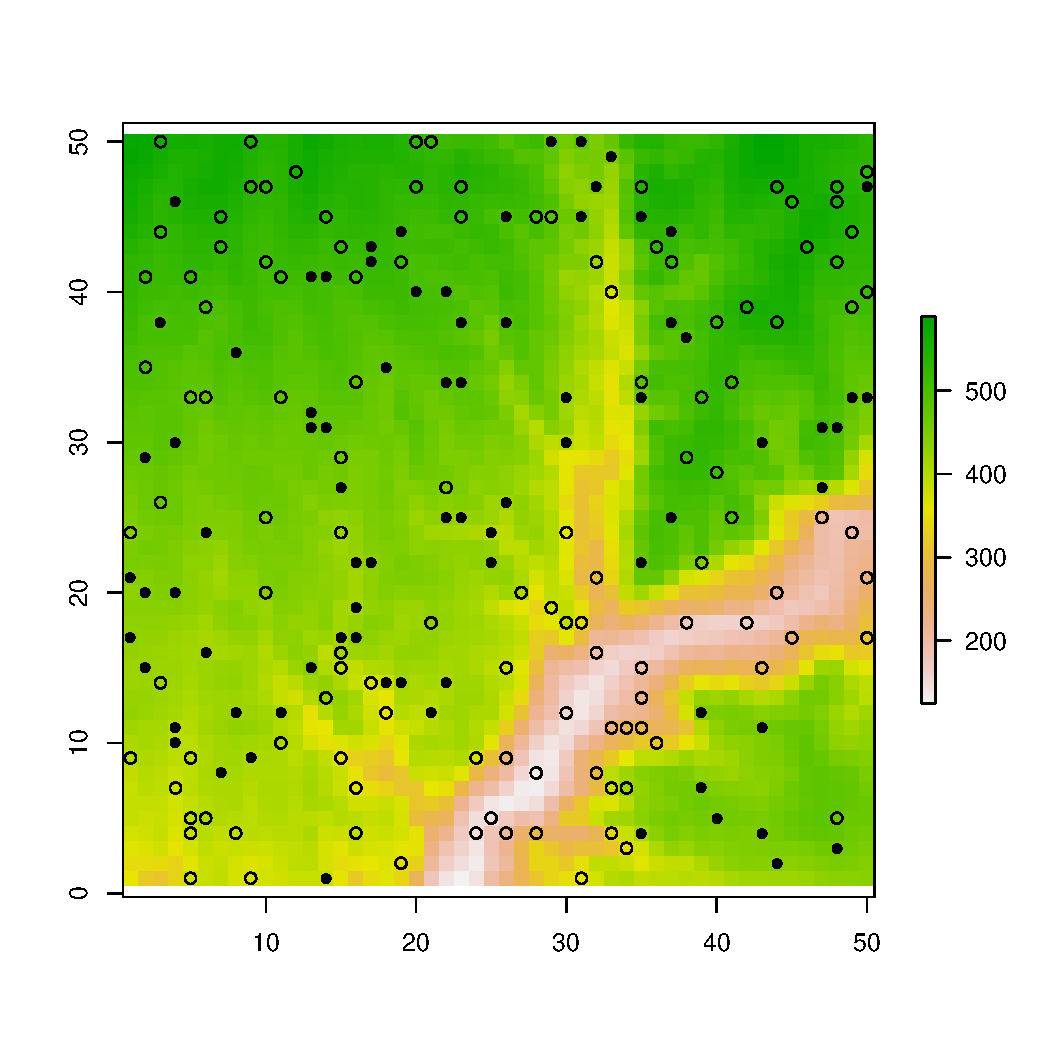
\includegraphics[width=8cm]{figures/observations-binomial.pdf}
  \caption{\textbf{Observation points}. Presences (full circles) and absences (empty
    circles) are localized on the altitude map (in m).}
  \label{fig:observations-binomial}
\end{figure}

\subsubsection{Parameter inference using the \texttt{hSDM.binomial()} function}

The \texttt{hSDM.binomial()} function performs a Binomial logistic regression in a Bayesian
framework. Before using this function we need to prepare a bit the data for parameter
inference and prediction. For parameter inference, we add the quadatric term for altitude
in the data frame associated to observations.

\begin{knitrout}\small
\definecolor{shadecolor}{rgb}{0.969, 0.969, 0.969}\color{fgcolor}\begin{kframe}
\begin{alltt}
\hlstd{data.obs}\hlopt{$}\hlstd{alt2} \hlkwb{<-} \hlstd{(data.obs}\hlopt{$}\hlstd{alt)}\hlopt{^}\hlnum{2}
\end{alltt}
\end{kframe}
\end{knitrout}


We want to have predictions on the whole landscape, not only at observation points. To
directly obtain these predictions, we can create a data frame including altitude data on
the whole landscape. This data frame will be used for the \texttt{suitability.pred}
argument. The data frame for predictions must include the same column names as those used
in the formula for the \texttt{suitability} argument (i.e. 'alt' and 'alt2' in our
example).

\begin{knitrout}\small
\definecolor{shadecolor}{rgb}{0.969, 0.969, 0.969}\color{fgcolor}\begin{kframe}
\begin{alltt}
\hlstd{data.pred} \hlkwb{<-} \hlkwd{data.frame}\hlstd{(}\hlkwc{alt}\hlstd{=}\hlkwd{values}\hlstd{(alt),}\hlkwc{alt2}\hlstd{=(}\hlkwd{values}\hlstd{(alt))}\hlopt{^}\hlnum{2}\hlstd{)}
\end{alltt}
\end{kframe}
\end{knitrout}


We can now call the \texttt{hSDM.binomial()} function. Setting parameter \texttt{save.p}
to 1, we can save in memory the MCMC values for predictions. These values can be used to compute
several statistics for each predictions (mean, median, 95\% quantiles). For example, mean
and 95\% quantiles are useful to estimate the uncertainty around the mean predictions.     

\begin{knitrout}\small
\definecolor{shadecolor}{rgb}{0.969, 0.969, 0.969}\color{fgcolor}\begin{kframe}
\begin{alltt}
\hlstd{mod.hSDM.binomial} \hlkwb{<-} \hlkwd{hSDM.binomial}\hlstd{(}\hlkwc{presences}\hlstd{=data.obs}\hlopt{$}\hlstd{Y,}
                                   \hlkwc{trials}\hlstd{=data.obs}\hlopt{$}\hlstd{trials,}
                                   \hlkwc{suitability}\hlstd{=}\hlopt{~}\hlstd{alt}\hlopt{+}\hlstd{alt2,}
                                   \hlkwc{data}\hlstd{=data.obs,}
                                   \hlkwc{suitability.pred}\hlstd{=data.pred,}
                                   \hlkwc{burnin}\hlstd{=}\hlnum{1000}\hlstd{,} \hlkwc{mcmc}\hlstd{=}\hlnum{1000}\hlstd{,} \hlkwc{thin}\hlstd{=}\hlnum{1}\hlstd{,}
                                   \hlkwc{beta.start}\hlstd{=}\hlnum{0}\hlstd{,}
                                   \hlkwc{mubeta}\hlstd{=}\hlnum{0}\hlstd{,} \hlkwc{Vbeta}\hlstd{=}\hlnum{1.0E6}\hlstd{,}
                                   \hlkwc{seed}\hlstd{=}\hlnum{1234}\hlstd{,} \hlkwc{verbose}\hlstd{=}\hlnum{1}\hlstd{,} \hlkwc{save.p}\hlstd{=}\hlnum{1}\hlstd{)}
\end{alltt}
\end{kframe}
\end{knitrout}


\subsubsection{Analysis of the results}

The \texttt{hSDM.binomial()} function returns an MCMC (Markov chain Monte Carlo) for each
parameter of the model and also for the model deviance. To obtain parameter estimates,
MCMC values can be summarized through a call to the \texttt{summary()} function from the
\textbf{coda} package. We can check that the values of the target parameters
$\beta_0=1$, $\beta_1=2$ and $\beta_2=-4$ are within the 95\% confidence interval of
the parameter estimates.

\begin{knitrout}\small
\definecolor{shadecolor}{rgb}{0.969, 0.969, 0.969}\color{fgcolor}\begin{kframe}
\begin{alltt}
\hlkwd{summary}\hlstd{(mod.hSDM.binomial}\hlopt{$}\hlstd{mcmc)}
\end{alltt}
\begin{verbatim}
## 
## Iterations = 1001:2000
## Thinning interval = 1 
## Number of chains = 1 
## Sample size per chain = 1000 
## 
## 1. Empirical mean and standard deviation for each variable,
##    plus standard error of the mean:
## 
##                     Mean    SD Naive SE Time-series SE
## beta.(Intercept)   0.887 0.226  0.00715         0.0236
## beta.alt           2.164 0.457  0.01445         0.0583
## beta.alt2         -4.133 0.606  0.01917         0.0958
## Deviance         189.821 2.172  0.06870         0.1433
## 
## 2. Quantiles for each variable:
## 
##                    2.5%     25%     50%    75%  97.5%
## beta.(Intercept)   0.45   0.739   0.889   1.05   1.28
## beta.alt           1.24   1.855   2.187   2.48   2.98
## beta.alt2         -5.22  -4.575  -4.153  -3.73  -2.93
## Deviance         187.38 188.271 189.234 190.77 195.52
\end{verbatim}
\end{kframe}
\end{knitrout}


Parameters estimates can be compared to results obtained with the \texttt{glm()} function.

\begin{knitrout}\small
\definecolor{shadecolor}{rgb}{0.969, 0.969, 0.969}\color{fgcolor}\begin{kframe}
\begin{alltt}
\hlcom{#== glm results for comparison}
\hlstd{mod.glm} \hlkwb{<-} \hlkwd{glm}\hlstd{(}\hlkwd{cbind}\hlstd{(Y,trials}\hlopt{-}\hlstd{Y)}\hlopt{~}\hlstd{alt}\hlopt{+}\hlstd{alt2,}\hlkwc{family}\hlstd{=}\hlstr{"binomial"}\hlstd{,}\hlkwc{data}\hlstd{=data.obs)}
\hlkwd{summary}\hlstd{(mod.glm)}
\end{alltt}
\begin{verbatim}
## 
## Call:
## glm(formula = cbind(Y, trials - Y) ~ alt + alt2, family = "binomial", 
##     data = data.obs)
## 
## Deviance Residuals: 
##    Min      1Q  Median      3Q     Max  
## -1.710  -0.787  -0.002   0.810   2.208  
## 
## Coefficients:
##             Estimate Std. Error z value Pr(>|z|)    
## (Intercept)    0.925      0.249    3.71  0.00021 ***
## alt            2.147      0.548    3.91  9.0e-05 ***
## alt2          -4.137      0.727   -5.69  1.3e-08 ***
## ---
## Signif. codes:  0 '***' 0.001 '**' 0.01 '*' 0.05 '.' 0.1 ' ' 1
## 
## (Dispersion parameter for binomial family taken to be 1)
## 
##     Null deviance: 269.20  on 199  degrees of freedom
## Residual deviance: 187.19  on 197  degrees of freedom
## AIC: 193.2
## 
## Number of Fisher Scoring iterations: 8
\end{verbatim}
\end{kframe}
\end{knitrout}


MCMC can also be graphically summarized with a call to the \texttt{plot.mcmc()} function,
also in the \textbf{coda} package. MCMC are plotted with a trace of the sampled output and
a density estimate for each variable in the chain (Fig.~\ref{fig:mcmc-binomial}). This can
plot can be used to visually check that the chains have converged.

\begin{knitrout}\small
\definecolor{shadecolor}{rgb}{0.969, 0.969, 0.969}\color{fgcolor}\begin{kframe}
\begin{alltt}
\hlkwd{plot}\hlstd{(mod.hSDM.binomial}\hlopt{$}\hlstd{mcmc)}
\end{alltt}
\end{kframe}
\end{knitrout}


\begin{figure}[!h] 
  \centering 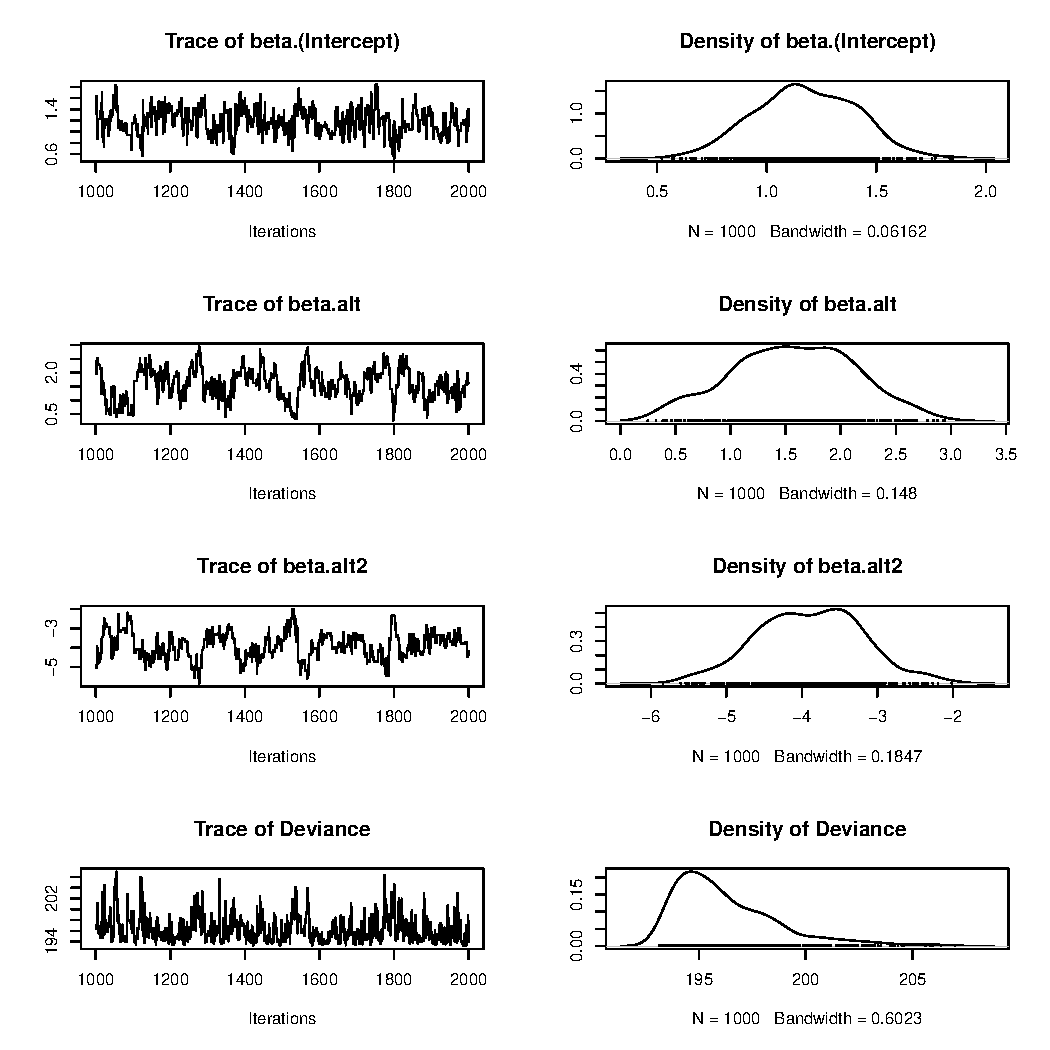
\includegraphics[width=\textwidth]{figures/mcmc-binomial.pdf}
  \caption{\textbf{Trace and density estimate for each variable of the MCMC}.}
  \label{fig:mcmc-binomial}
\end{figure}

The \texttt{hSDM.binomial()} function also returns two other objects. The first one,
\texttt{prob.p.latent}, is the predictive posterior mean of the latent variable
$\theta$ (the probability of presence) for each observation. 

\begin{knitrout}\small
\definecolor{shadecolor}{rgb}{0.969, 0.969, 0.969}\color{fgcolor}\begin{kframe}
\begin{alltt}
\hlkwd{str}\hlstd{(mod.hSDM.binomial}\hlopt{$}\hlstd{prob.p.latent)}
\end{alltt}
\begin{verbatim}
##  num [1:200] 0.34 0.689 0.14 0.271 0.76 ...
\end{verbatim}
\begin{alltt}
\hlkwd{summary}\hlstd{(mod.hSDM.binomial}\hlopt{$}\hlstd{prob.p.latent)}
\end{alltt}
\begin{verbatim}
##    Min. 1st Qu.  Median    Mean 3rd Qu.    Max. 
##   0.000   0.111   0.414   0.397   0.689   0.761
\end{verbatim}
\end{kframe}
\end{knitrout}


The second one, \texttt{prob.p.pred} is the set of sampled values from the predictive
posterior (if parameter \texttt{save.p} is set to 1) or the predictive posterior mean (if
\texttt{save.p} is set to 0) for each prediction. In our example, \texttt{save.p} is set
to 1 and \texttt{prob.p.pred} is an \texttt{mcmc} object. Values in \texttt{prob.p.pred} can be
used to plot the predicted probability of presence on the whole landscape and the
uncertainty associated to the predictions (Fig~\ref{fig:predictions-binomial}).

\begin{knitrout}\small
\definecolor{shadecolor}{rgb}{0.969, 0.969, 0.969}\color{fgcolor}\begin{kframe}
\begin{alltt}
\hlcom{# Create a raster for predictions}
\hlstd{theta.pred.mean} \hlkwb{<-} \hlkwd{raster}\hlstd{(theta)}
\hlcom{# Create rasters for uncertainty}
\hlstd{theta.pred.2.5} \hlkwb{<-} \hlstd{theta.pred.97.5} \hlkwb{<-} \hlkwd{raster}\hlstd{(theta)}
\hlcom{# Attribute predicted values to raster cells}
\hlstd{theta.pred.mean[]} \hlkwb{<-} \hlkwd{apply}\hlstd{(mod.hSDM.binomial}\hlopt{$}\hlstd{prob.p.pred,}\hlnum{2}\hlstd{,mean)}
\hlstd{theta.pred.2.5[]} \hlkwb{<-} \hlkwd{apply}\hlstd{(mod.hSDM.binomial}\hlopt{$}\hlstd{prob.p.pred,}\hlnum{2}\hlstd{,quantile,}\hlnum{0.025}\hlstd{)}
\hlstd{theta.pred.97.5[]} \hlkwb{<-} \hlkwd{apply}\hlstd{(mod.hSDM.binomial}\hlopt{$}\hlstd{prob.p.pred,}\hlnum{2}\hlstd{,quantile,}\hlnum{0.975}\hlstd{)}
\hlcom{# Plot the predicted probability of presence and uncertainty}
\hlkwd{plot}\hlstd{(theta.pred.mean,}\hlkwc{col}\hlstd{=}\hlkwd{rev}\hlstd{(}\hlkwd{heat.colors}\hlstd{(}\hlnum{255}\hlstd{)))}
\hlkwd{plot}\hlstd{(theta.pred.2.5,}\hlkwc{col}\hlstd{=}\hlkwd{rev}\hlstd{(}\hlkwd{heat.colors}\hlstd{(}\hlnum{255}\hlstd{)))}
\hlkwd{plot}\hlstd{(theta.pred.97.5,}\hlkwc{col}\hlstd{=}\hlkwd{rev}\hlstd{(}\hlkwd{heat.colors}\hlstd{(}\hlnum{255}\hlstd{)))}
\end{alltt}
\end{kframe}
\end{knitrout}


\begin{figure}[!h] 
  \centering 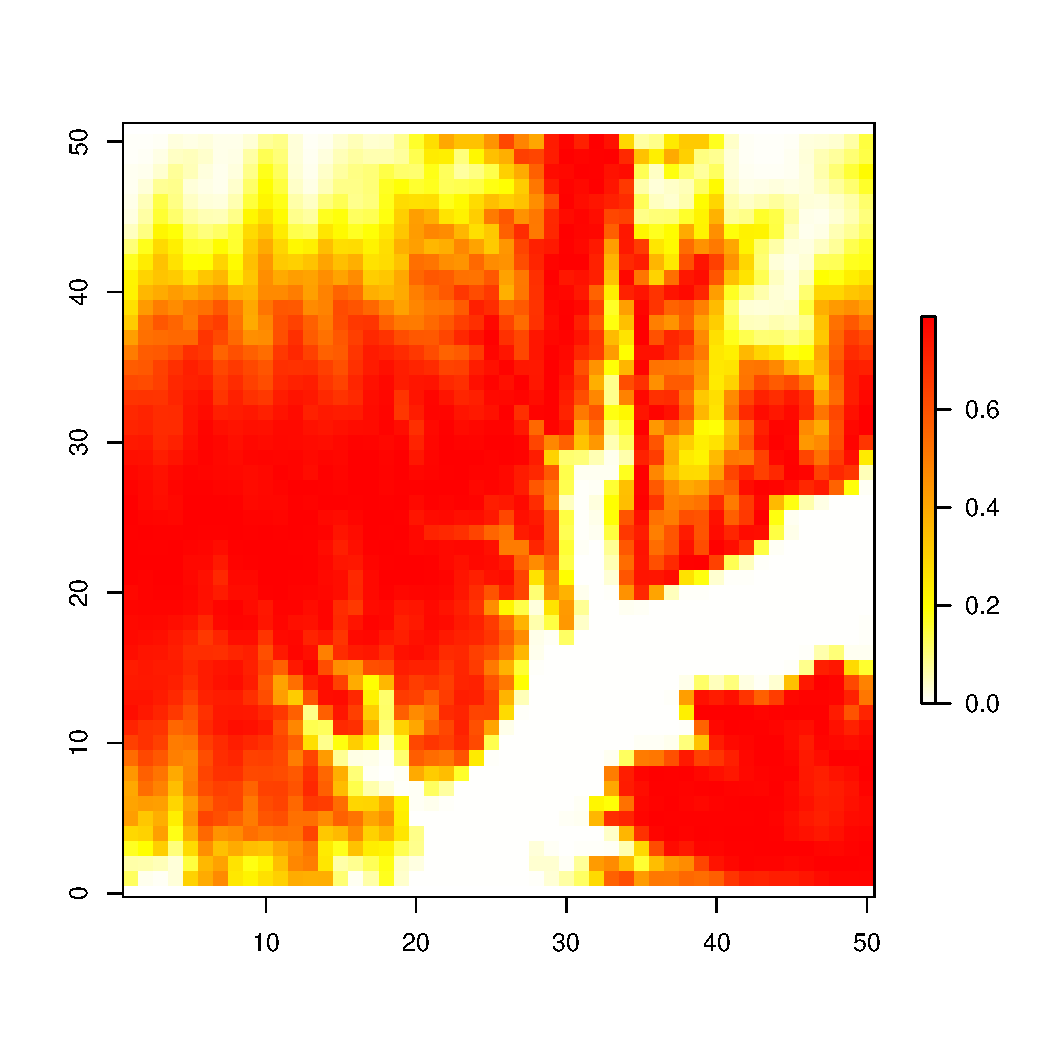
\includegraphics[width=8cm]{figures/predictions-binomial1.pdf} \\
  \begin{tabular}{cc}
    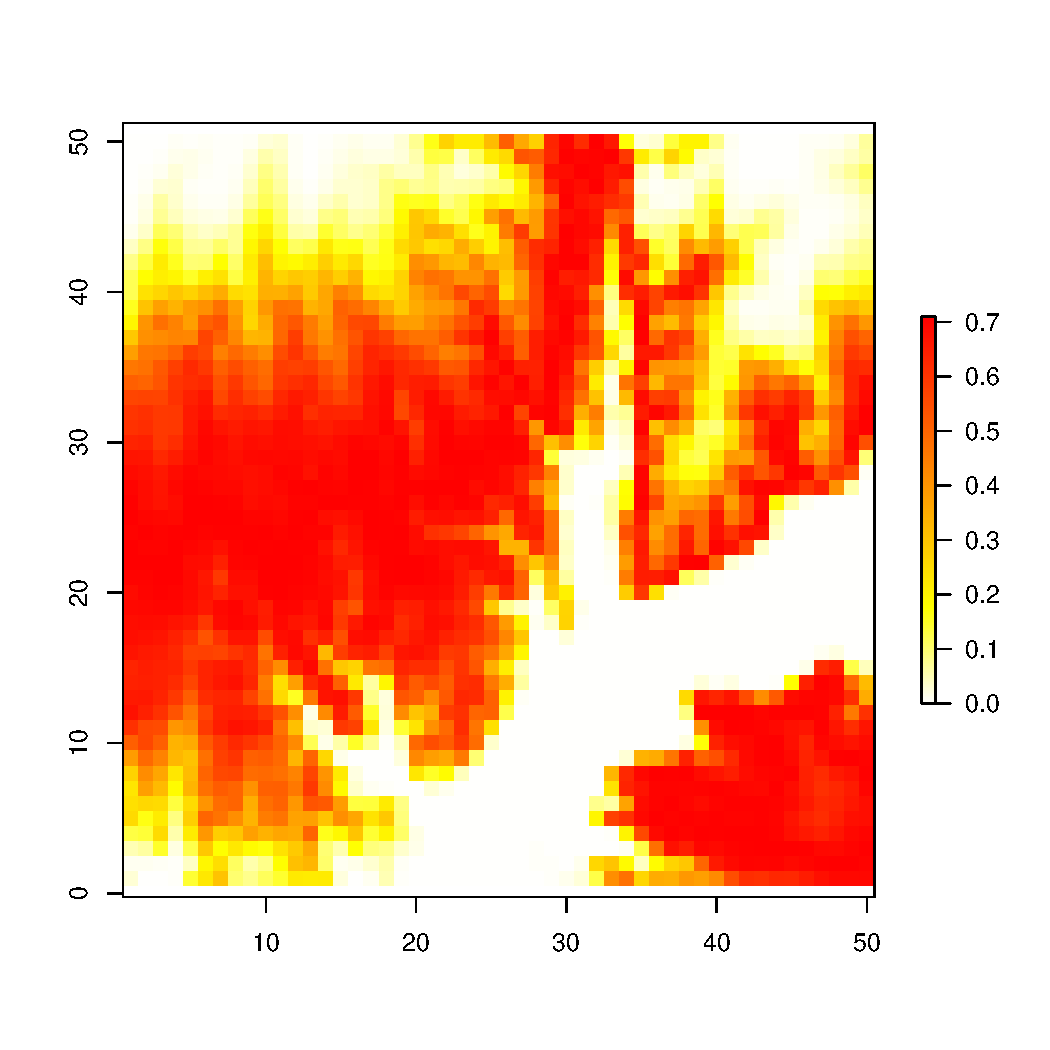
\includegraphics[width=8cm]{figures/predictions-binomial2.pdf} &
    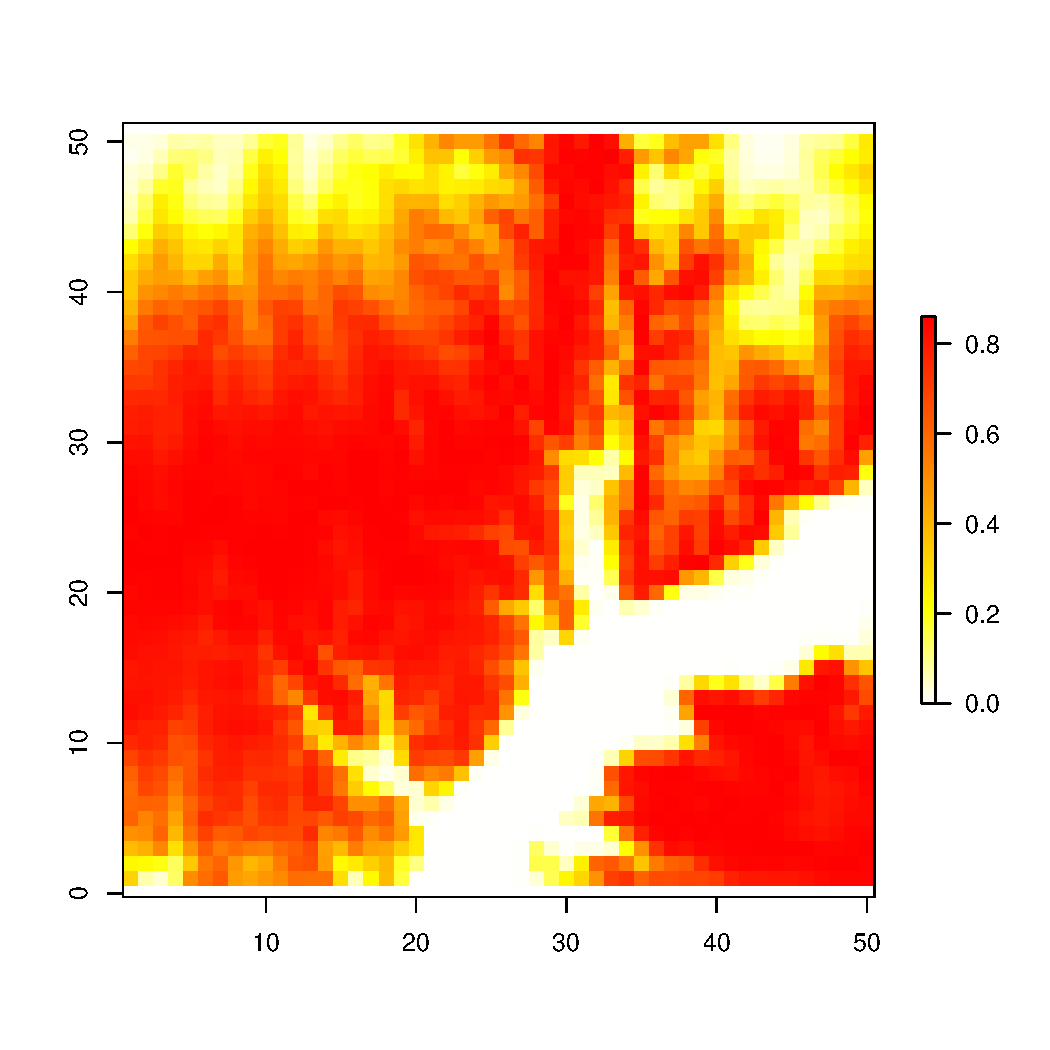
\includegraphics[width=8cm]{figures/predictions-binomial3.pdf} \\
  \end{tabular}
  
  \caption{\textbf{Predicted probability of presence and uncertainty of predictions}. Mean
    probability of presence (top), predictions at 2.5\% quantile (bottom left) and 97.5\%
    quantile (bottom right) can be plotted from the \texttt{mcmc} object
    \texttt{plot.p.pred} returned by function \texttt{hSDM.binomial()}.}
  
  \label{fig:predictions-binomial}
  
\end{figure}

In our example, we can compare the predictions to the initial probability of presence
computed from our model to check that our predictions are correct
(Fig.~\ref{fig:pred-obs-binomial}).

\begin{knitrout}\small
\definecolor{shadecolor}{rgb}{0.969, 0.969, 0.969}\color{fgcolor}\begin{kframe}
\begin{alltt}
\hlcom{# Comparing predictions to initial values}
\hlkwd{plot}\hlstd{(theta[],theta.pred.mean[],}\hlkwc{cex.lab}\hlstd{=}\hlnum{1.4}\hlstd{)}
\hlkwd{abline}\hlstd{(}\hlkwc{a}\hlstd{=}\hlnum{0}\hlstd{,}\hlkwc{b}\hlstd{=}\hlnum{1}\hlstd{,}\hlkwc{col}\hlstd{=}\hlstr{"red"}\hlstd{,}\hlkwc{lwd}\hlstd{=}\hlnum{2}\hlstd{)}
\end{alltt}
\end{kframe}
\end{knitrout}


\begin{figure}[!h] 
  \centering 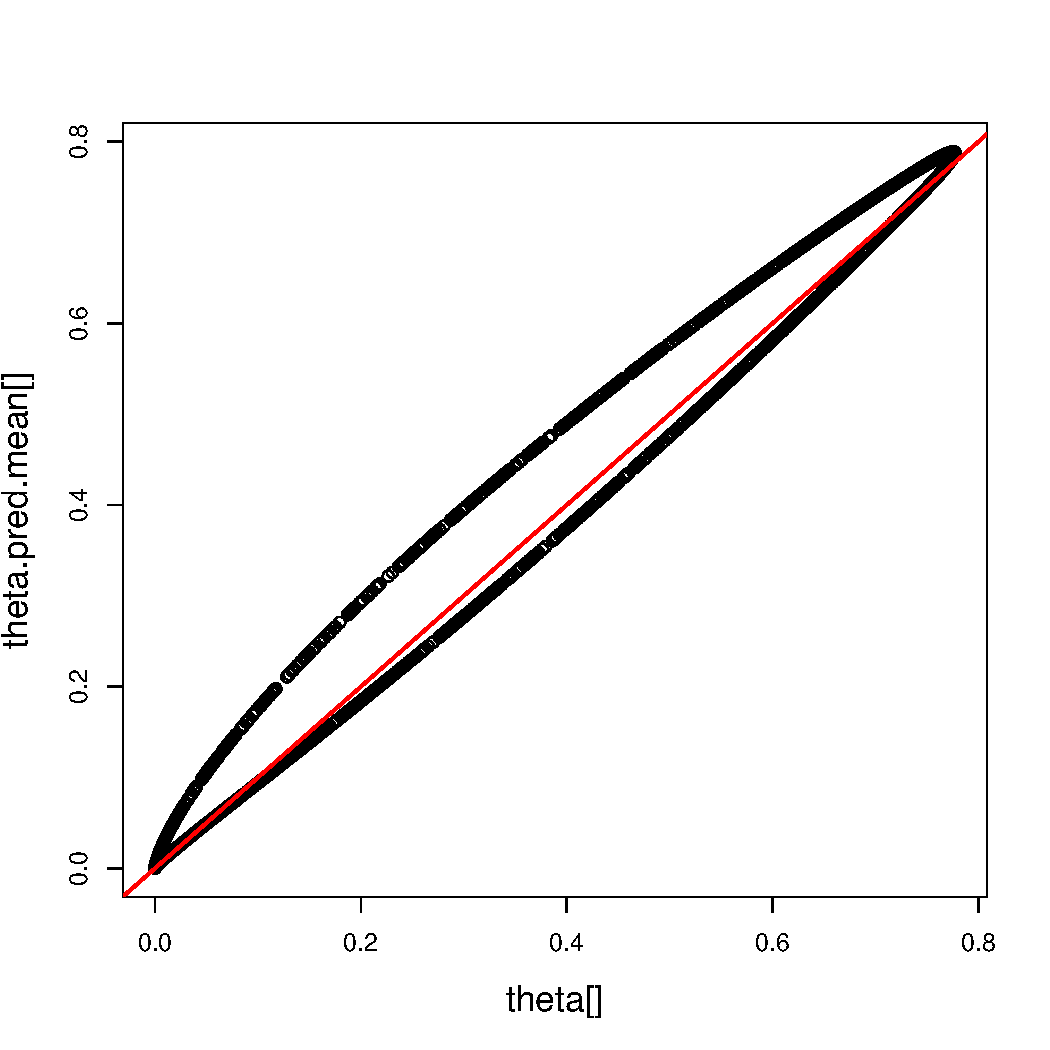
\includegraphics[width=8cm]{figures/pred-obs-binomial.pdf}
  
  \caption{\textbf{Predicted vs. initial probabilities of presence}. Initial probabilities
    of presence are computed from the Binomial logistic regression model with fixed
    parameters.}
  
  \label{fig:pred-obs-binomial}
  
\end{figure}

\end{document}
